%%%%%%%%%%%%%%%%%%%%%%%%%%%%%%%%%%%%%%%%%%%%%%%%%%%%%%%%%%%%%%%%%%%%%%%%%%%
%                                                                         %
%           TEMPLATE LATEX PER TESI                                       %
%           ______________                                                %
%                                                                         %
%           Ultima revisione: 24 giugno 2019                              %
%           Revisori: G.Presti; L.A.Ludovico; F. Avanzini                 %
%                                                                         %
%%%%%%%%%%%%%%%%%%%%%%%%%%%%%%%%%%%%%%%%%%%%%%%%%%%%%%%%%%%%%%%%%%%%%%%%%%%

\documentclass[12pt,italian]{report}
\usepackage{tesi}

% CORSO DI LAUREA:
\def\myCDL{Corso di Laurea triennale in Informatica}

% TITOLO TESI:
\def\myTitle{Pattern di assegnamento ottimizzati per l'efficienza energetica in edge computing}

% AUTORE:
\def\myName{Manuel Parati}
\def\myMat{Matr. 958584}

% RELATORE E CORRELATORE:
\def\myRefereeA{Prof. Alberto Ceselli}
\def\myRefereeB{Prof. Marco Premoli}

% ANNO ACCADEMICO
\def\myYY{2021-2022}

% Il seguente comando introduce un elenco delle figure dopo l'indice
%\figurespagetrue

% Il seguente comando introduce un elenco delle tabelle dopo l'indice
%\tablespagetrue

%
%       PREAMBOLO
%       Inserire qui eventuali package da includere o definizioni di comandi personalizzati
%

% Package di formato
\usepackage[a4paper]{geometry}      % Formato del foglio
\usepackage[italian]{babel}         % Supporto per l'italiano
\usepackage[utf8]{inputenc}         % Supporto per UTF-8
%\usepackage[a-1b]{pdfx}            % File conforme allo standard PDF-A (obbligatorio per la consegna)

% Package per la grafica
\usepackage{graphicx}               % Funzioni avanzate per le immagini
\usepackage{hologo}                 % Bibtex logo with \hologo{BibTeX}
\usepackage{epsfig}                % Permette immagini in EPS
%\usepackage{xcolor}                % Gestione avanzata dei colori

% Package tipografici
\usepackage{amssymb,amsmath,amsthm} % Simboli matematici
\usepackage{listings}               % Scrittura di codice

% Package ipertesto
\usepackage{url}                    % Visualizza e rendere interattii gli URL
\usepackage{hyperref}               % Rende interattivi i collegamenti interni

% Package algoritmi
\usepackage{algorithm,algpseudocode}

% Package appendice
\usepackage[toc,page]{appendix}

\numberwithin{equation}{section}    % Numerazione delle equazione indicando la sezione
\allowdisplaybreaks                 % Permette di spezzare i modelli quanto necessario

% Permette di avere "Input" e "Output" negli algoritmi invece di "Require" e "Ensure"
\renewcommand{\algorithmicrequire}{\textbf{Input:}}
\renewcommand{\algorithmicensure}{\textbf{Output:}}

% Definisce il testo da inserire nei riferimenti agli algoritmi
\newcommand{\algorithmautorefname}{algoritmo}

% Permette di avere la scritta "Appendici" invece di "Appendices".
\renewcommand{\appendixpagename}{Appendici}
\renewcommand{\appendixtocname}{Appendici}

% Permette di avere "Algoritmo" nella caption.
\floatname{algorithm}{Algoritmo}

% Permette di fare riferimenti alle righe degl algoritmi.
\makeatletter
\patchcmd{\ALG@step}{\addtocounter{ALG@line}{1}}{\refstepcounter{ALG@line}}{}{}
\newcommand{\ALG@lineautorefname}{linea}
\makeatother


\begin{document}

% Creazione automatica del frontespizio
\frontespizio
\beforepreface

%
%       RINGRAZIAMENTI
%

\prefacesection{Ringraziamenti}
Questa sezione, contiene i ringraziamenti.

%
%       Creazione automatica dell'indice
%

\afterpreface

% 
%       CAPITOLI
% 

\chapter{Introduzione}
\label{cap:introduzione}

\dots


%
%   OBBIETTIVI
%
\section{Obbiettivi}
\label{sec:obbiettivi}

\dots


%
%   ORGANIZZAZIONE ELABORATO
%
\section{Struttura dell'elaborato}
\label{sec:organizzazione-elaborato}

\dots

\chapter{Modellazione del sistema}
\label{cap:modellazione-sistema}

Questo capitolo fornisce una panoramica riguardo all'infrastruttura Mobile Edge Computing ed illustra il modello di orchestrazione proposto in questo lavoro.


%
%   INFRASTRUTTURA MEC
%
\section{L'infrastruttura Mobile Edge Computing}
\label{sec:infrastruttura-mec}

All'interno di un'infrastruttura Mobile Edge Computing (MEC) si trovano i cluster di virtualizzazione, spesso noti come `MEC facility' o più semplicemente `facility', e gli access point (AP). Le facility sono il luogo in cui avviene la virtualizzazione e sono composte dalle macchine virtuali (VM) su cui si eseguono le applicazioni degli utenti finali, mentre gli AP sono i dispositivi (per esempio le antenne wireless) a cui gli end point si collegano per poter ricevere il servizio. Ogni AP è associato ad una facility, a cui inoltra tutto il traffico che riceve: questo significa che ogni facility avrà in esecuzione nelle proprie VM tutte le applicazioni utilizzate dagli utenti connessi agli AP a lui associati. Ogni facility, per poter gestire il traffico che le viene inoltrato, deve utilizzare una quantità di energia direttamente proporzionale a tale domanda. Per questo motivo, ognuna di esse possiede dei pannelli fotovoltaici che generano una quantità di energia variabile nel tempo, dipendente dal numero di pannelli installati e dall'irraggiamento a cui sono sottoposti. L'energia prodotta può essere direttamente utilizzata oppure immagazzinata all'interno di alcune batterie, dotate di capacità limitata. Nel caso in cui l'energia disponibile, data dalla somma tra quella accumulata e quella generata, non basti a soddisfare la domanda, è possibile acquistarne altra ad un prezzo dipendente dalla facility e dall'istante temporale.

Data la natura mobile degli end point, che sono per esempio smartphone o laptop, il traffico a cui sono sottoposti gli AP varia nel tempo e di conseguenza cambia la domanda rivolta alle facility. Per questo motivo l'assegnamento viene effettuato dinamicamente, e lo strumento incaricato di svolgere tale compito è l'orchestratore, che implementa la logica definita dal modello di orchestrazione. Le azioni che svolge vengono chiamate `orchestrazioni' o `switch' e consistono nell'assegnare un AP ad una facility diversa da quella attuale, provocando il ridimensionamento della potenza delle VM in termini del numero di processori e memoria disponibile, e la migrazione del loro stato. Il ridimensionamento è dovuto alla variazione di domanda da gestire, mentre la migrazione dello stato è necessaria per avere in esecuzione in ogni facility le applicazioni utilizzate dagli utenti connessi agli AP che le sono assegnati. Il costo prodotto dalla migrazione prende il nome di `costo di migrazione'.

\begin{figure}[t]
    \centering
    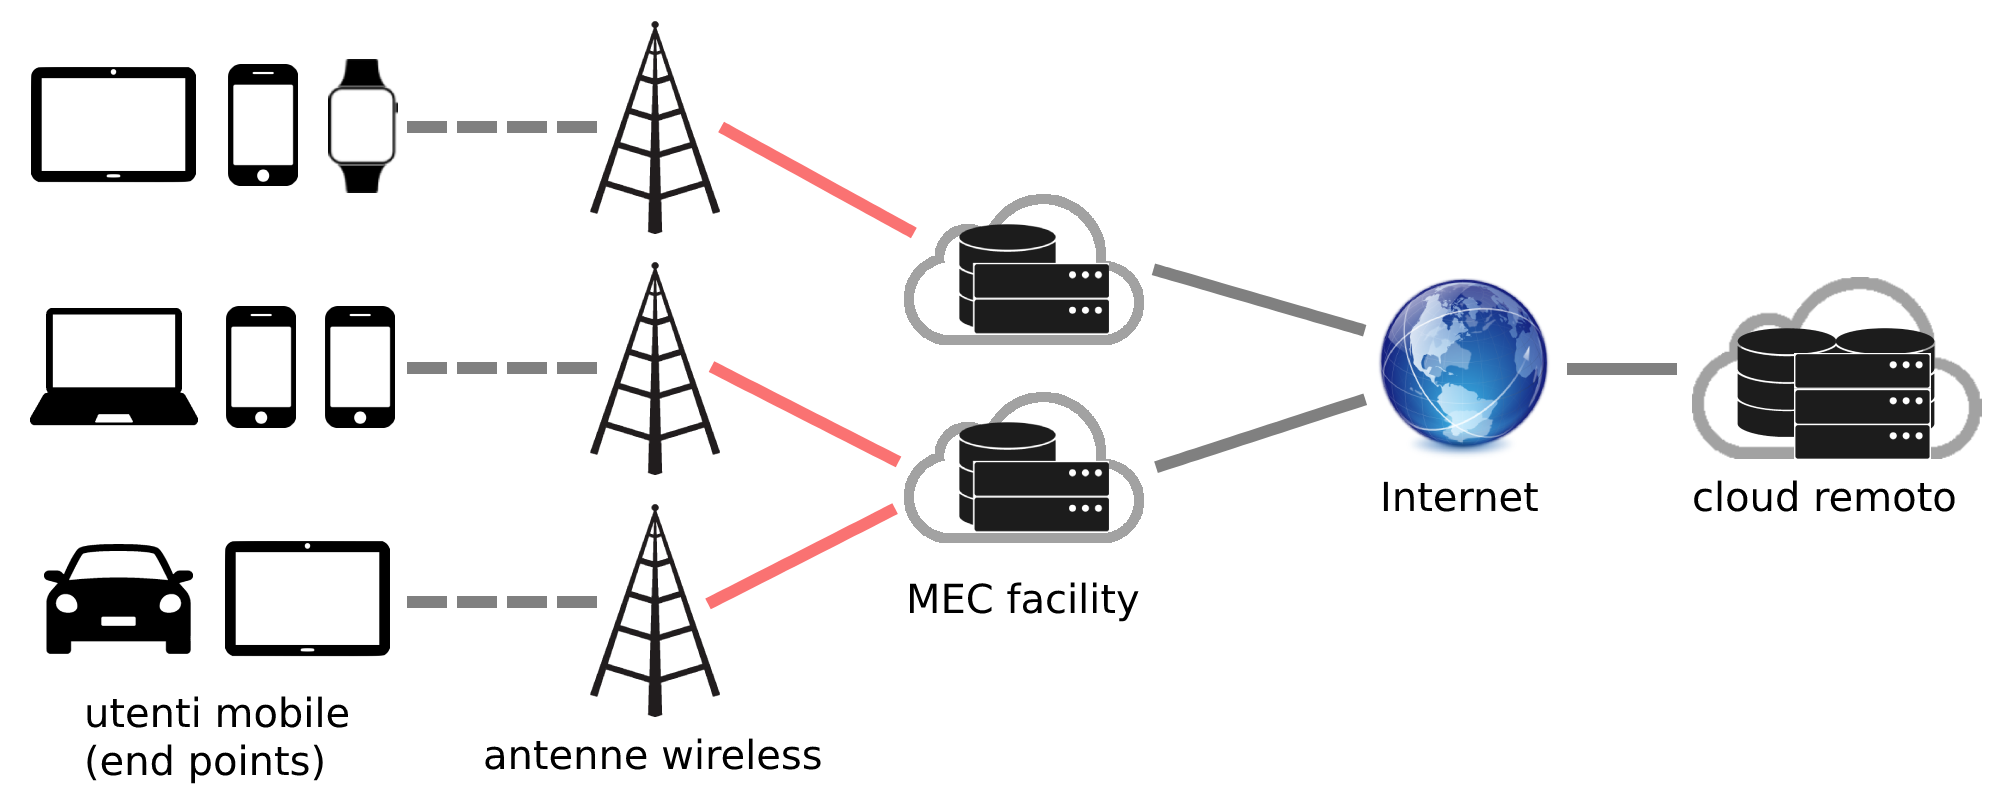
\includegraphics[width = 150mm]{img/esempio-infrastruttura-mec.jpg}
    \caption{Esempio di un'infrastruttura Mobile Edge Computing (MEC).}
    \label{fig:architettura-mec}
\end{figure}

Nella \autoref{fig:architettura-mec} è presente un'infrastruttura MEC composta da due facility e tre AP, a cui sono collegati diversi dispositivi mobili di vario genere. Si noti come ogni dispositivo invii il proprio traffico all'AP a cui è collegato, e come tutto il traffico ricevuto da ogni AP sia inoltrato alla stessa facility. Si può osservare, per esempio, come al secondo AP siano connessi un laptop e due smartphone, mentre al terzo un'automobile smart ed un tablet. Nella figura i due AP sono assegnati alla stessa facility (la seconda) che riceverà e dovrà quindi gestire il traffico di tutti e cinque i dispositivi. Si noti infine come sia presente un cloud centralizzato che gestisce e sincronizza le varie facility.


%
%   INFRASTRUTTURA MEC
%
\section{Modello di orchestrazione proposto}
\label{sec:modello-di-orchestrazione-proposto}

Il modello di orchestrazione proposto rappresenta una variante di quello presentato negli articoli \cite{assignment-patterns} e \cite{analytics-mec}, in cui nell'effettuare le scelte di orchestrazione si tiene in considerazione anche l'utilizzo dell'energia da parte delle facility.

Come illustrato in \cite{analytics-mec}, all'interno del modello viene introdotta una discretizzazione temporale che permette di effettuare migrazioni solo in determinati istanti, per esempio ogni 15 minuti. Questa scelta è ragionevole, dato che in caso contrario si pagherebbe un costo troppo elevato in termini di migrazione e spese generali dovute alla gestione del traffico. L'orizzonte temporale viene quindi rappresentato da un insieme di time-slot della stessa durata.

L'obbiettivo del modello è quello di effettuare assegnamenti che permettano di raggiungere un buon compromesso tra: ottenere una buona qualità del servizio (cioè bassa latenza per l'utente finale), costi di migrazione contenuti e buona gestione dell'energia da parte delle facility. Nell'effettuare le scelte bisogna tenere in considerazione che la domanda degli AP e l'energia prodotta dalle facility varia nel corso del tempo, e che ogni facility possiede un limite massimo di domanda che è in grado di soddisfare simultaneamente e una quantità di energia limite che può mantenere nello stesso momento all'interno delle proprie batterie. Si supponga inoltre che le facility, per gestire una unità di traffico, debbano utilizzare una unità di energia.

\begin{figure}[t]
    \centering
    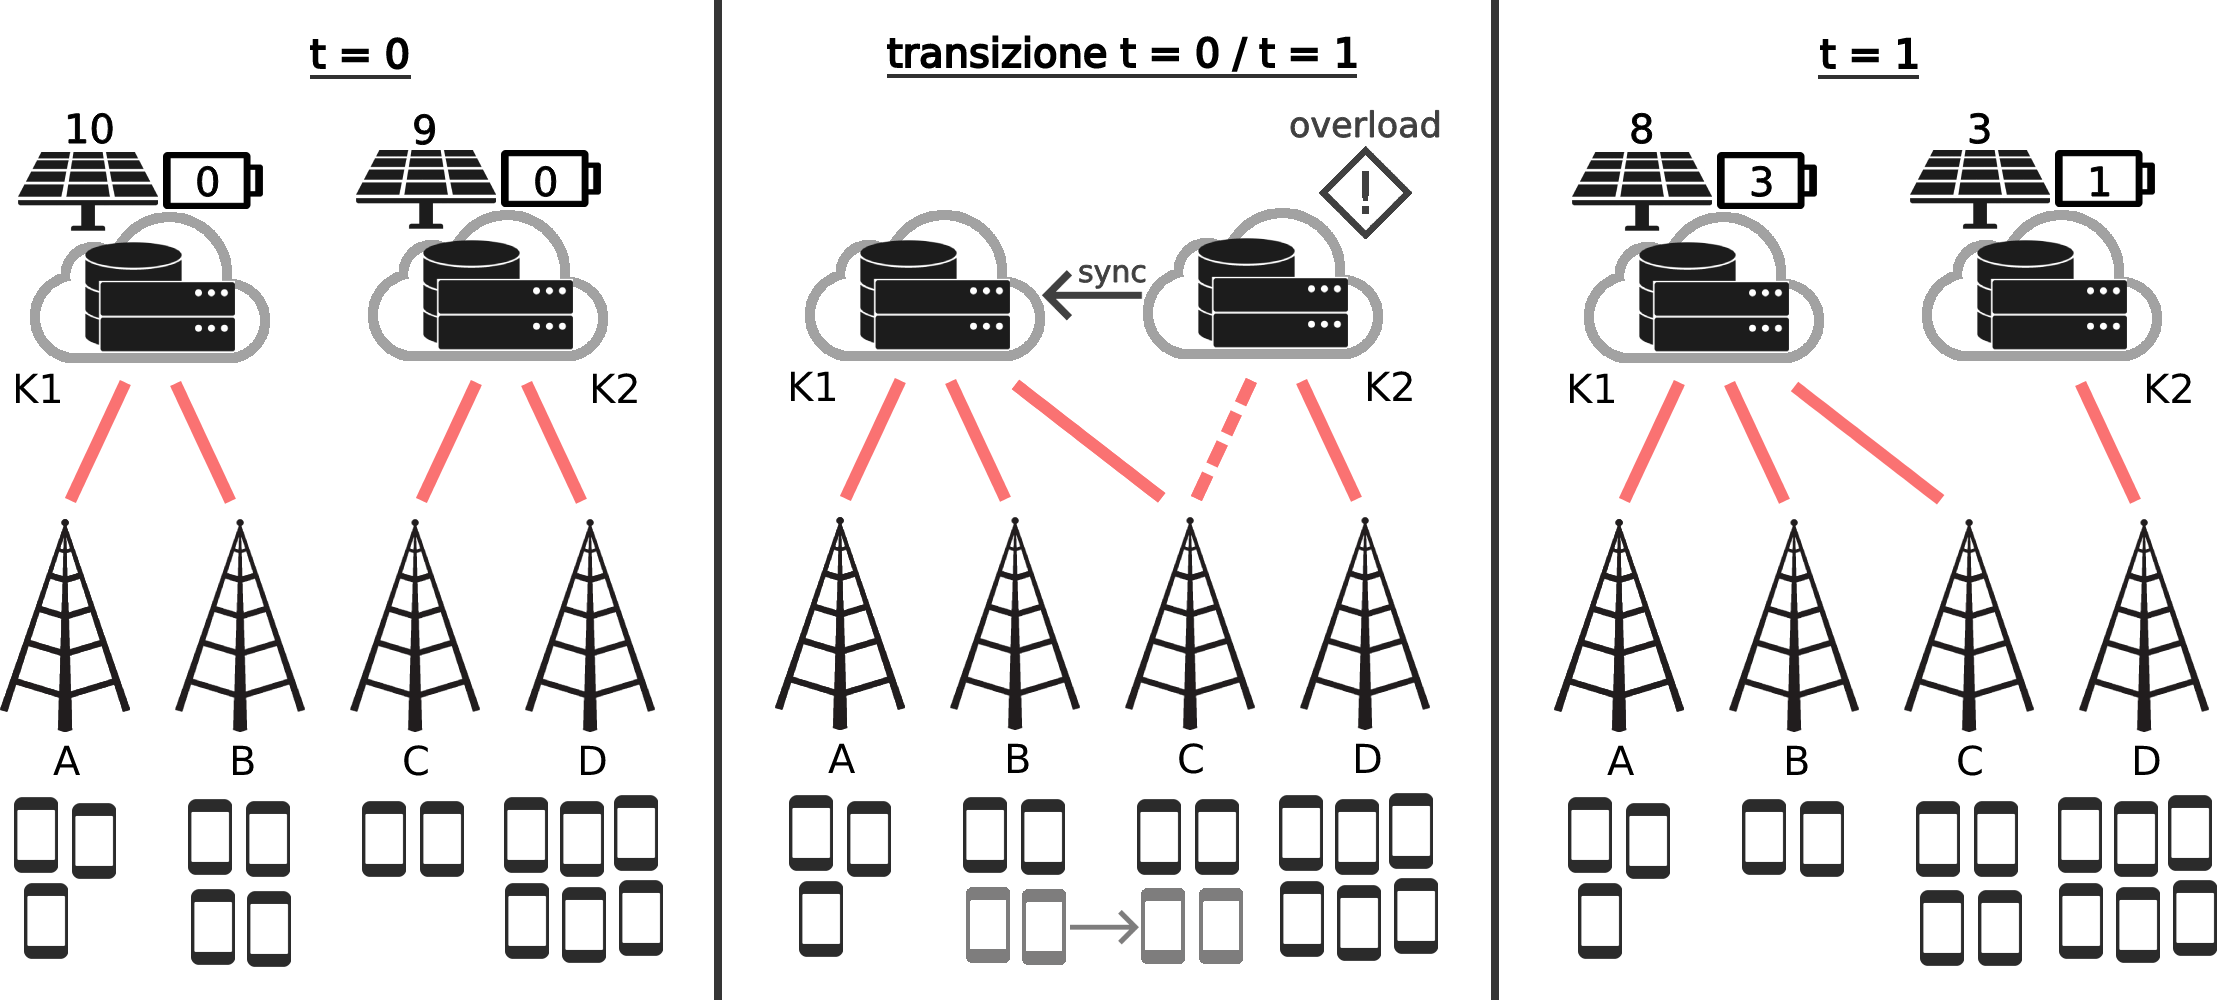
\includegraphics[width = 150mm]{img/esempio-assegnamenti.jpg}
    \caption{Esempio funzionamento del modello di orchestrazione.}
    \label{fig:esempio-assegnamenti}
\end{figure}


%
%   ESEMPIO FUNZIONAMENTO
%
\subsection{Esempio del funzionamento}
\label{sub-sec:esempio-funzionamento}

Una semplice applicazione di esempio è presentata nella \autoref{fig:esempio-assegnamenti}. Come si può osservare, è presente una rete MEC con due facility (\texttt{K1} e \texttt{K2}) e quattro AP (\texttt{A}, \texttt{B}, \texttt{C}, \texttt{D}) considerata in due time-slot consecutivi (\texttt{t}=0, 1). Gli end point connessi agli AP sono rappresentati con dei piccoli rettangoli, e si supponga che inizialmente le batterie siano vuote in entrambe le facility. Nel primo time-slot (\texttt{t}=1) gli AP \texttt{A} e \texttt{B} sono associati alla facility \texttt{K1} mentre \texttt{C} e \texttt{D} a \texttt{K2}, quindi tutti gli utenti che sono connessi ad \texttt{A} e \texttt{B} avranno le proprie applicazioni in esecuzione su una VM presente in \texttt{K1}, mentre quelli connessi a \texttt{C} e \texttt{D} le avranno in \texttt{K2}. Questi assegnamenti permettono di avere una buona latenza dato che ogni AP è connesso alla facility più vicina, ma anche una buona gestione energetica, in quanto nella facility \texttt{K1} vengono prodotte 10 unità di energia ed utilizzate solo 7 mentre in \texttt{K2} se ne producono 9 e utilizzano 8. In entrambi i casi avanzano delle unità (3 in \texttt{K1} e 1 in \texttt{K2}) che vengono immagazzinate nelle batterie per poter essere spese nei prossimi time-slot. Successivamente due utenti connessi all'AP \texttt{B} si spostano e si agganciano a \texttt{C}: a questo punto \texttt{K2} riceve una richiesta di domanda eccessiva che non riesce a gestire e di conseguenza è necessario effettuare un'orchestrazione per ribilanciare il traffico. Questo comporta l'assegnare \texttt{C} a \texttt{K1}, ridimensionare le VM (aumentarne la potenza in \texttt{K1} e diminuirla in \texttt{K2}) e sincronizzare le facility trasferendo lo stato delle VM riguardanti tutti gli utenti connessi a \texttt{C} da \texttt{K2} a \texttt{K1}. In un contesto reale, il modello deve prevenire una situazione di questo tipo effettuando orchestrazioni che tengano in considerazione la futura domanda dei vari AP, dato che questa circostanza va ad inficiare la qualità complessiva del servizio. Nel secondo time-slot (\texttt{t}=1) si avranno quindi gli AP \texttt{A}, \texttt{B} e \texttt{C} assegnati alla facility \texttt{K1}, mentre \texttt{D} a \texttt{K2}. Dal punto di vista energetico, la facility \texttt{K1} riesce a soddisfare la domanda di traffico (9 unità) utilizzando l'energia presente nella batteria e quella prodotta in questo time-slot (8 + 3 unità complessive). Per quanto riguarda invece \texttt{K2}, l'energia disponibile (3 + 1 unità) non è sufficiente e quindi è necessario acquistare 6 ulterione unità. Da notare come l'energia potrebbe avere costi diversi nel corso dei time-slot, e di conseguenza potrebbe risultare conveniente acquistarla quando il costo è basso per immagazzinarla ed utilizzarla successivamente.


%
%   IMPLEMENTAZIONE
%
\subsection{Implementazione}
\label{sub-sec:implementazione}

Il comportamento del modello di orchestrazione fin qui descritto viene implementato attraverso un modello di programmazione lineare chiamato `modello di assegnamento dinamico' e descritto dettagliatamente nella \autoref{sec:modello-completo}. Al modello viene fornita come input un'instanza del problema (formata dati dati riguardanti l'infrastruttura MEC presa in considerazione e, per ogni time-slot, il traffico rivolto agli AP e la produzione di energia di ogni facility) e ritorna in output il piano degli assegnamenti ottimale. Questa rappresenta la miglior metodologia per risolvere il problema in quanto garantisce di ottenere la soluzione ottima, ma a causa della sua natura combinatoria potrebbe essere inutilizzabile in deterimnate situazioni. Infatti quando il numero di time-slot presi in considerazione oppure la quantità di AP o facility aumenta, il tempo di calcolo necessario ad arrivare alla soluzione ottima cresce esponenzialmente fino a diventare proibitivo. Per questo motivo vengono successivamente proposte due euristiche, che semplificano il problema con l'obbiettivo di abbassare la complessità del modello ed ottenere una soluzione non troppo peggiore rispetto a quella ottima. Nella \autoref{sec:semplificazione-modello} viene presentata la prima idea euristica, che mira ad abbassare la complessità semplificando il modello utilizzato, mentre nella \autoref{sec:aggregamento-time-slot} la seconda, che aggrega i time-slot dell'istanza per ottenerne una più facilmente risolvibile.

\chapter{Modelli di ottimizzazione}
\label{cap:modelli-ottimizzazione}

In questo capitolo vengono introdotti i modelli di ottimizzazione utilizzati nel corso dell'elaborato. Nel primo sottocapitolo si illustra il modello di assegnamento dinamico rappresentante il problema descritto, mentre nei due successivi quelli utilizzati dagli algoritmi euristici: il modello di assegnamento statico ed il modello che effettua l'assegnamento utilizzando istanze composte da un solo time-slot.


%
%   MODELLO COMPLETO
%
\section{Modello di assegnamento dinamico}
\label{sec:modello-completo}

Il `modello di assegnamento dinamico' è un modello di programmazione lineare misto-intera (MILP) che, considerata un'infrastruttura MEC, è in grado di definire dinamicamente gli assegnamenti AP-facility all'interno di un arco temporale in cui sono noti i livelli di traffico rivolti agli AP e l'energia prodotta dalle facility, per ogni time-slot. Con `dinamicamente' si intende la possibilità di assegnare lo stesso AP a facility differenti nel corso dei time-slot, permettento di bilanciare nel tempo la domanda complessiva rivolta alle facility. Questo migliora la latenza complessiva e la gestione energetica attuata, ma provoca la necessità di dover gestire i vari switch e pagare i costi di migrazione. L'output del modello è un piano degli assegnamenti: viene indicato in ogni time-slot a quale facility della rete deve indirizzare il traffico ogni AP. Di conseguenza è possibile estrarre anche il piano delle orchestrazioni, che corrisponde ad un valore booleano per ogni time-slot, per ogni AP e per ogni coppia di facility, che assume come valore `vero' se in quell'instante temporale l'AP effettua uno switch tra le facility considerate, altrimenti `falso'.

\paragraph*{Dati.}

Data un'infrastruttura MEC, siano $A$ l'insieme degli AP e $K$ l'insieme delle facility che la compongono. Si supponga inoltre di avere un orizzonte temporale discretizzato in un insieme di $T$ time-slot. Vengono indicati, per ogni AP $i \in A$, con $d^t_i$ la quantità di traffico a cui $i$ è sottoposto al time-slot $t \in T$ e con $m_{i,k}$ la distanza fisica tra $i$ e la facility $k \in K$. La distanza di rete tra due facility $j, k \in K \times K$ è invece denotata con $l_{jk}$: tale valore è direttamente proporzionale alla loro distanza fisica ed alla latenza di rete, includendo anche il tempo necessario a processare i pacchetti all'interno dei nodi intermedi. Data una facility $k \in K$, siano: $C_k$ la quantità di domanda che riesce a gestire contemporaneamente, $G_k$ la capienza complessiva delle sue batterie, $p_k$ l'energia inizialmente presente all'interno delle batterie, $e^t_k$ l'energia che produce nel time-slot $t \in T$, e $c^t_k$ il prezzo a cui può acquistare l'energia nel time-slot $t \in T$.

\paragraph*{Variabili.}

Siano $x^t_{ik}$ variabili binarie che assumono valore 1 nel caso in cui al time-slot $t \in T$ l'AP $i \in A$ è assegnato alla facility $k \in K$, altrimenti 0. Le variabili $y^t_{ijk}$ sono anch'esse binarie e valgono 1 se l'AP $i \in A$ viene associato alla facility $j \in K$ al tempo $t - 1$ ed alla facility $k \in K$ al tempo $t$, altrimenti 0. Da notare come queste siano le variabili che indicano le orchestrazioni da effettuare. Per ogni facility $k \in K$ e time-slot $t \in T$, siano: $g^t_k$ l'energia residua della facility $k$ al tempo $t$ (quindi quella che viene immagazzinata all'interno delle batterie e disponibile nel time-slot $t+1$), $v^t_k$ l'energia utilizzata dalla facility $k$ al tempo $t$ e $z^t_k$ la quantità di energia acquistata dalla facility $k$ al tempo $t$.

\paragraph*{Modello.}

Di seguito la rappresentazione matematica del modello.

\begin{align}
    \min\quad       & \alpha \sum_{t \in T} \sum_{i \in A} \sum_{\substack{(j,k) \in \\ K \times K}}d^{t}_{i} l_{jk} y^t_{ijk} + \beta \sum_{t \in T} \sum_{i \in A} \sum_{k \in K}d^{t}_{i} m_{ik} x^t_{ik} + \gamma \sum_{t \in T} \sum_{k \in K}{c_k^t z_k^t}
    \label{eq:complete-obj}
\end{align}
\vspace*{-6mm}
\begin{align}
    \text{s.t.\quad}
    \label{eq:complete-c1}
    & v_k^t = \sum_{i \in A}{d^t_i x_{ik}^t}        &   & \forall k \in K, \forall t \in T                                  \\
    \label{eq:complete-c2}
    & \sum_{k \in K}{x_{ik}^t} = 1                  &   & \forall i \in A, \forall t \in T                                  \\
    \label{eq:complete-c3}
    & x_{ik}^t = \sum_{l \in K}{y_{ilk}^t}          &   & \forall i \in A, \forall k \in K, \forall t \in T \setminus \{1\} \\
    \label{eq:complete-c4}
    & x_{ik}^t = \sum_{l \in K}{y_{ikl}^{t+1}}      &   & \forall i \in A, \forall k \in K, \forall t \in T \setminus \{T\} \\
    \label{eq:complete-c5}
    & z_k^1 + e_k^1 + p_k \geq v_k^1 + g_k^1        &   & \forall k \in K                                                   \\
    \label{eq:complete-c6}
    & z_k^t + e_k^t + g_k^{t-1} \geq v_k^t + g_k^t  &   & \forall k \in K, \forall t \in T \setminus \{1\}                  \\
    \label{eq:complete-c7}
    & g_k^t \leq G_k                                &   & \forall k \in K, \forall t \in T                                  \\
    \label{eq:complete-c8}
    & v_k^t \leq C_k                                &   & \forall k \in K, \forall t \in T                                  \\
    \label{eq:complete-c9}
    & x_{ik}^t \in \{0,1\}                          &   & \forall i \in A, \forall k \in K, \forall t \in T                 \\
    \label{eq:complete-c10}
    & y_{ik'k''}^t \in \{0,1\}                      &   & \forall i \in A, \forall k', k'' \in K, \forall t \in T           \\
    \label{eq:complete-c11}
    & x, y, g, v, z \geq 0                          &   &
\end{align}


\paragraph*{Obbiettivo.}

La funzione obbiettivo (\ref{eq:complete-obj}) ha lo scopo di ottenere la soluzione che possiede il miglior bilanciamento tra avere una buona latenza per l'utente finale ed ottenere costi di migrazione e di acquisto dell'energia contenuti. In particolare, si vuole minimizzare la somma tra (nell'ordine) i costi complessivi di migrazione, la latenza complessiva e il costo globale di acquisto dell'energia, dove i parametri $\alpha$, $\beta$ e $\gamma$ indicano quanto peso dare a ciascun componente.

\paragraph*{Vincoli.}

I vincoli \ref{eq:complete-c1} determinano il valore delle variabili $v^t_k$: la domanda a cui è sottoposta la facility $k \in K$ al tempo $t \in T$ è data dalla somma del traffico proveniente da tutti gli AP che le sono assegnati in quel time-slot. I vincoli \ref{eq:complete-c2} impongono ogni AP ad essere assegnato esattamente ad una facility per time-slot. I vincoli \ref{eq:complete-c3} e \ref{eq:complete-c4} collegano le variabili $x$ ed $y$ e servono a gestire il flusso degli switch: quando $x^t_{ik}$ vale 0 significa che l'AP $i \in A$ non è associato alla facility $k \in K$ e di conseguenza non permettono di effettuare nessuna orchestrazione, mentre nel caso contrario impongono di effettuarne esattamente una oppure mantenere l'AP $i$ associato alla facility $k$. I vincoli \ref{eq:complete-c5} e \ref{eq:complete-c6} gestiscono il flusso dell'energia: impongono che per ogni time-slot e per ogni facility la quantità di energia disponibile (data dalla somma tra quella prodotta, quella presente nelle batterie e quella acquistata) sia non minore della somma tra la quantità utilizzata e quella che viene immagazzinata nelle batterie. I vincoli \ref{eq:complete-c7} e \ref{eq:complete-c8} limitano superiormente i valori che possono assumere rispettivamente le variabili $g$ e $v$, facendo in modo che non venga sforata la capienza delle batterie e la capacità delle facility.


%
%   MODELLO MIGRAZIONI A INF
%
\section{Modello di assegnamento statico}
\label{sec:modello-migrazioni-inf}

Il `modello di assegnamento statico' è un modello di tipo MILP che ha lo stesso scopo del modello di assegnamento dinamico (\ref{sec:modello-completo}) ma con la differenza che non permette di effettuare switch. Ogni AP sarà quindi assegnato alla stessa facility per tutto l'arco temporale preso in considerazione, e non attuando migrazioni il costo di migrazione complessivo sarà 0. In generale, utilizzare un approccio di assegnamento dinamico fornisce minore latenza e migliore efficienza energetica complessive rispetto ad uno statico, in quanto è possibile adattare gli assegnamenti alla variazione del traffico richiesto dai vari AP ed alla quantità di energia prodotta dalle facility. La formulazione del problema statico è però più leggera rispetto alla controparte dinamica, infatti necessita di un numero inferiore di variabili e vincoli, con conseguente diminuzione della complessità combinatoria. L'output del modello in questo caso sarà una lista di assegnamenti validi per tutti i time-slot.

\paragraph*{Dati.}

I dati su cui opera sono gli stessi del modello dinamico, si veda la \autoref{sec:modello-completo} per una panoramica completa.

\paragraph*{Variabili.}

Siano $x_{ik}$ variabili binarie che assumono valore 1 se l'AP $i \in A$ viene assegnato alla facility $k \in K$, 0 altrimenti. Per ogni facility $k \in K$ e per ogni time-slot $t \in T$ siano inoltre $g^t_k$ l'energia residua della facility $k$ al tempo $t$, $v^t_k$ l'energia utilizzata dalla facility $k$ al tempo $t$ e $z^t_k$ la quantità di energia acquistata dalla facility $k$ al tempo $t$. Come si può notare, il set di variabili viene notevolmente ridotto rispetto al modello dinamico, in quanto imponendo assegnamenti statici non è più necessario gestire il flusso degli switch e memorizzare gli assegnamenti per ogni time-slot. Le variabili $y$ diventano quindi superflue, e per determinare gli assegnamenti è sufficiente una variabile $x$ per ogni coppia AP-facility.

\paragraph*{Modello.}

Di seguito la rappresentazione matematica del modello.

\begin{align}
    \min\quad       & \beta \sum_{t \in T} \sum_{i \in A} \sum_{k \in K}{d^t_i m_{ik} x_{ik}} + \gamma \sum_{t \in T} \sum_{k \in K}{c_k^t z_k^t}
    \label{eq:migrinf-obj}
\end{align}
\vspace*{-10mm}
\begin{align}
    \text{s.t.\quad}
    \label{eq:migrinf-c1}
    & \sum_{i \in A}{d^t_i x_{ik}} = v_k^t          &   & \forall k \in K, \forall t \in T                 \\
    \label{eq:migrinf-c2}
    & \sum_{k \in K}{x_{ik}} = 1                    &   & \forall i \in A                                  \\
    \label{eq:migrinf-c3}
    & z_k^1 + e_k^1 + p_k \geq v_k^1 + g_k^1        &   & \forall k \in K                                  \\
    \label{eq:migrinf-c4}
    & z_k^t + e_k^t + g_k^{t-1} \geq v_k^t + g_k^t  &   & \forall k \in K, \forall t \in T \setminus \{1\} \\
    \label{eq:migrinf-c5}
    & g_k^t \leq G_k                                &   & \forall k \in K, \forall t \in T                 \\
    \label{eq:migrinf-c6}
    & v_k^t \leq C_k                                &   & \forall k \in K, \forall t \in T                 \\
    \label{eq:migrinf-c7}
    & x_{ik} \in \{0,1\}                            &   & \forall i \in A, \forall k \in K                 \\
    \label{eq:migrinf-c8}
    & x, g, v, z \geq 0                             &   &
\end{align}


\paragraph*{Obbiettivo.}

La funzione obbiettivo (\ref{eq:migrinf-obj}) ha lo scopo di determinare la soluzione che rappresenta il miglior compromesso tra ottenere una bassa latenza complessiva e un prezzo totale di acquisto dell'energia contenuto. I parametri $\beta$ e $\gamma$ corrispondono ai pesi da assegnare a ciascuna componente. Da notare come l'unica differenza con la funzione del modello normale (\ref{eq:complete-obj}) sia l'assenza della prima parte, riguardante i costi di migrazione.

\paragraph*{Vincoli.}

I vincoli \ref{eq:migrinf-c1} determinano il valore delle variabili $v^t_k$: l'energia utilizzata dalla facility $k \in K$ al tempo $t \in T$ è data dalla somma del traffico proveniente da ogni AP $i \in A$ che le è assegnato; mentre i vincoli \ref{eq:migrinf-c2} impongono ad ogni AP di essere associato esattamente ad una facility. I vincoli \ref{eq:migrinf-c3} e \ref{eq:migrinf-c4} riguardano la gestione ed il flusso dell'energia e sono equivalenti ai \ref{eq:complete-c5} e \ref{eq:complete-c6} del modello dinamico, mentre quelli rappresentati dalle disequazioni \ref{eq:migrinf-c5} e \ref{eq:migrinf-c6} impongono di non eccedere rispettivamente la capacità delle batterie e la capienza delle facility, e sono l'equivalente dei \ref{eq:migrinf-c7} e \ref{eq:migrinf-c8}.


\subsection{Variante con quadro energetico completo}

Da notare come questo modello non garantisca di tracciare il reale flusso di energia che avviene all'interno delle facility, dato che per come sono posti i vincoli \ref{eq:migrinf-c3} e \ref{eq:migrinf-c4} ci potrebbero essere delle quantità di energia residua che non vengono accumulate in quanto non utilizzate nei time-slot successivi. Nel determinare la soluzione ottima questo non causa problemi, ma nei casi in cui si necessita di un quadro realistico della gestione energetica, è necessario apportare alcune modifiche. In particolare, si deve immagazzinare ogni volta tutta l'energia possibile, quindi i vincoli \ref{eq:migrinf-c3} e \ref{eq:migrinf-c4} vengono rispettivamente riformulati come:
\begin{align}
    \label{eq:statico-c3var}
    & z_k^1 + e_k^1 + p_k = v_k^1 + g_k^1 + s_k^1       &   & \forall k \in K                                  \\
    \label{eq:statico-c4var}
    & z_k^t + e_k^t + g_k^{t-1} = v_k^t + g_k^t + s_k^t &   & \forall k \in K, \forall t \in T \setminus \{1\}
\end{align}
\noindent
dove $s^t_k$ sono variabili non negative che indicano la quantità di energia non accumulabile nella facility $k \in K$ al tempo $t \in T$ a causa della capienza limitata delle batterie. La quantità di energia disponibile (data dalla somma tra quella acquistata, quella prodotta e quella presente nelle batterie) è posta quindi uguale alla somma tra la quantità utilizzata, la quantità accumulata e la quantità non accumulabile. A questo punto nella funzione obbiettivo (\ref{eq:migrinf-obj}) è necessario minimizzare anche la somma complessiva dell'energia non accumulabile ($\sum_{t \in T}\sum_{k \in K} s^t_k$), trasformandola in:
\begin{align}
    \label{eq:migrinf-objvar}
    \min\quad       & \beta \sum_{t \in T} \sum_{i \in A} \sum_{k \in K}{d^t_i m_{ik} x_{ik}} + \gamma \sum_{t \in T} \sum_{k \in K}{c_k^t z_k^t} + \sum_{t \in T} \sum_{k \in K}{s_k^t}
\end{align}
\noindent
in modo tale da avere nelle variabili $g$ il valore più alto possibile, e quindi immagazzinare ogni volta tutta la quantità possibile.

Di seguito la rappresentazione matematica completa:

\begin{align}
    \tag{\ref*{eq:statico-objvar}}
    \min\quad       & \beta \sum_{t \in T} \sum_{i \in A} \sum_{k \in K}{d^t_i m_{ik} x_{ik}} + \gamma \sum_{t \in T} \sum_{k \in K}{c_k^t z_k^t} + \sum_{t \in T} \sum_{k \in K}{s_k^t}
\end{align}
\vspace*{-6mm}
\begin{align}
    \text{s.t.\quad}
    \tag{\ref*{eq:statico-c1}}
    & v_k^t = \sum_{i \in A}{d^t_i x_{ik}}              &   & \forall k \in K, \forall t \in T                 \\
    \tag{\ref*{eq:statico-c2}}
    & \sum_{k \in K}{x_{ik}} = 1                        &   & \forall i \in A                                  \\
    \tag{\ref*{eq:statico-c3var}}
    & z_k^1 + e_k^1 + p_k = v_k^1 + g_k^1 + s_k^1       &   & \forall k \in K                                  \\
    \tag{\ref*{eq:statico-c4var}}
    & z_k^t + e_k^t + g_k^{t-1} = v_k^t + g_k^t + s_k^t &   & \forall k \in K, \forall t \in T \setminus \{1\} \\
    \tag{\ref*{eq:statico-c5}}
    & g_k^t \leq G_k                                    &   & \forall k \in K, \forall t \in T                 \\
    \tag{\ref*{eq:statico-c6}}
    & v_k^t \leq C_k                                    &   & \forall k \in K, \forall t \in T                 \\
    \tag{\ref*{eq:statico-c7}}
    & x_{ik} \in \{0,1\}                                &   & \forall i \in A, \forall k \in K                 \\
    \label{eq:statico-c8}
    & x, g, v, z, s \geq 0                              &   &
\end{align}


Da notare come l'aggiunta delle variabili $s$ renda questo modello leggermente più complesso rispetto a quello di riferimento, e che nel risolvere le stesse istanze si otterranno risultati della stessa qualità.


%
%   MODELLO SINGOLO SLOT TIME
%
\section{Modello di assegnamento singolo time-slot}
\label{sec:modello-migrazioni-0}

Il `modello di assegnamento singolo time-slot' è un modello di tipo MILP ottimizzato per definire gli assegnamenti all'interno di istanze composte da un singolo time-slot, e fornisce quindi in output la facility a cui deve indirizzare il traffico ogni AP nel time-slot considerato.

\paragraph*{Dati.}

Data un'infrastruttura MEC, siano $A$ l'insieme degli AP e $K$ l'insieme delle facility che la compongono. Per ogni AP $i \in A$, vengono indicati con $d_i$ la quantità di traffico a cui $i$ è sottoposto e con $m_{ik}$ la distanza fisica tra $i$ e la facility $k \in K$. La distanza di rete tra due facility $j, k \in K \times K$ è invece denotata con $l_{jk}$: tale valore è direttamente proporzionale alla loro distanza fisica ed alla latenza di rete, incluso il tempo di processamento dei pacchetti nei nodi intermedi. Data una facility $k \in K$, siano: $C_k$ la quantità di domanda che riesce a gestire contemporaneamente, $p_k$ l'energia inizialmente presente all'interno delle sue batterie, $e_k$ l'energia che produce, e $c_k$ il prezzo a cui può acquistare l'energia.

\paragraph*{Variabili.}

Gli assegnamenti sono rappresentati da variabili binarie $x_{ik}$, che assumono come valore 1 se l'AP $i \in A$ viene assegnagno alla facility $k \in K$, altrimenti 0. Inoltre, data una facility $k \in K$, siano: $z_k$ l'energia che acquista, $v_k$ l'energia che utilizza e $s_k$ l'energia residua al termine del time-slot.

\paragraph*{Modello.}

\begin{align}
    \min\quad       & \beta \sum_{i \in A} \sum_{k \in K}{d_{i} m_{ik} x_{ik}} + \gamma \sum_{k \in K}{c_k z_k}
    \label{eq:migr0-obj}
\end{align}
\vspace*{-10mm}
\begin{align}
    \text{s.t.\quad}
    \label{eq:migr0-c1}
    & \sum_{i \in A}{d_i x_{ik}} = v_k              &   & \forall k \in K                  \\
    \label{eq:migr0-c2}
    & \sum_{k \in K}{x_{ik}} = 1                    &   & \forall i \in A                  \\
    \label{eq:migr0-c3}
    & z_k + e_k + p_k = v_k + g_k                   &   & \forall k \in K                  \\
    \label{eq:migr0-c4}
    & v_k \leq C_k                                  &   & \forall k \in K                  \\
    \label{eq:migr0-c5}
    & x_{ik} \in \{0,1\}                            &   & \forall i \in A, \forall k \in K \\
    \label{eq:migr0-c6}
    & a, x, p, v, z \geq 0                          &   &
\end{align}


\paragraph*{Obbiettivo.}

La funzione obbiettivo (\ref{eq:migr0-obj}) ha lo scopo di definire gli assegnamenti che rispecchiano il miglior trade-off tra l'ottenere una bassa latenza complessiva ed avere una spesa energetica contenuta. Da notare come prendendo in cosiderazione un singolo time-slot, non sia possibile effettuare switch e di conseguenza l'obbiettivo rispecchia quello presente nel modello di assegnamento statico (\ref{eq:migrinf-obj}).

\paragraph*{Vincoli.}

I vincoli \ref{eq:migr0-c1} definiscono il valore delle variabili $v_k$, mentre i \ref{eq:migr0-c2} impongono di assegnare ogni AP ad esattamente una facility. I vincoli \ref{eq:migr0-c3} gestiscono l'utilizzo dell'energia, mentre i \ref{eq:migr0-c4} definiscono un limite superiore alla quantità di traffico che ogni facility può gestire. Da notare come in questo caso, trattandosi di un singolo time-slot, non viene tenuta in considerazione la possibilità di immagazzinare l'energia nella batterie, e quindi tutta quelle le quantità in eccesso saranno indicate dalle variabili $s$.

\chapter{Algoritmi euristici}
\label{cap:algoritmi-euristici}

In questo capitolo vengono presentate le due euristiche proposte per semplificare il problema.

%
%   SEMPLIFICAZIONE MODELLO
%
\section{Euristica 1: semplificazione del modello}
\label{sec:semplificazione-modello}

Il primo algoritmo euristico proposto in questo lavoro si pone l'obbiettivo di ridurre la complessità del problema andando a semplificare il modello di ottimizzazione utilizzato. In particolare, l'idea è quella di effettuare le orchestrazioni solo in determinati time-slot prestabiliti, in modo tale da poter suddividere l'istanza considerata in sottoistanze all'interno delle quali ogni AP rimane associato alla stessa facility per tutto l'arco temporale: ciascuna di esse può quindi essere risolta indipendentemente utilizzando il modello di assegnamento statico, ed i vari risultati aggregati per formare il risultato originario. Da notare come le orchestrazioni sono una conseguenza dell'aver aggregato i risultati parziali, e che vengono quindi effettuate senza tener conto dei costi di migrazione che andranno pagati. Ciò significa che gli assegnamenti vanno ad ottimizzare solo la latenza ottenuta e la gestione energetica effettuata, ma dato che dovranno rimanere inalterati per diversi time-slot, ha senso pagare un costo maggiore nei pochi switch fatti pur di ottenere una migliore ottimizzazione complessiva.

\subsection{L'algoritmo}
\label{subsec:algo-model}

\begin{algorithm}
    \caption{Pseudocodice euristica 1}
    \label{alg:euristica-semplificazione-modello}
    \begin{algorithmic}[1]
        \Require l'istanza da risolvere, composta dagli insiemi $T$, $A$, $K$ e i dati $C$, $G$, $d$, $l$, $m$, $e$, $c$
        \Ensure il piano degli assegnamenti risultante, quindi il valore delle variabili $x$
        \State Siano $x, g, v, z, s$ le variabili del risultato globale
        \State $t \gets -1$
        \State $\operatorname{costo\_migrazione} \gets 0$
        \State $S \gets \operatorname{split}(T, A, K, C, G, d, l, m, e, c)$
        \For{$\textbf{all} ~ j \in \{0, \dots, |S|-1\}$}
            \State \{Siano $j$ considerati in ordine crescente\}
            \State $(\bar{T}$, $\bar{A}$, $\bar{K}, \bar{C}, \bar{G}, \bar{d}, \bar{l}, \bar{m}, \bar{e}, \bar{c}) \gets S[j]$
            \If{$j = 0$}
                \State $p_k \gets 0 ~ \forall k \in K$
            \Else
                \State $p_k \gets g^t_k ~ \forall k \in K$
            \EndIf
            \State $(\hat{x}, \hat{g}, \hat{v}, \hat{z}, \hat{s}) \gets \operatorname{calcola\_assegnamenti}(\bar{T}$, $\bar{A}$, $\bar{K}, \bar{C}, \bar{G}, \bar{d}, \bar{l}, \bar{m}, \bar{e}, \bar{c})$
            \If{$j > 0$}
                \For{$\textbf{all} ~ i \in A$}
                \State $k_{\operatorname{prec}} \gets \underset{k \in K}{\arg\max} ~ x^t_{ik}$
                \State $k_{\operatorname{succ}} \gets \underset{k \in K}{\arg\max} ~ \hat{x}^0_{ik}$
                    \If{$k_{\operatorname{prec}} \neq k_{\operatorname{succ}}$}
                        \State $\operatorname{costo\_migrazione} \gets \operatorname{costo\_migrazione} ~ + ~ d^t_i \cdot l_{k_{\operatorname{prev}} k_{\operatorname{succ}}}$
                    \EndIf
                \EndFor
            \EndIf
            \State $x \gets x \cup \hat{x}$
            \State $g \gets g \cup \hat{g}$
            \State $v \gets v \cup \hat{v}$
            \State $z \gets z \cup \hat{z}$
            \State $s \gets s \cup \hat{s}$
            \State $t \gets t + |T|$
        \EndFor
    \end{algorithmic}
\end{algorithm}


L'\autoref{alg:euristica-sempl} mostra le operazioni necessarie ad implementare l'idea euristica esposta. Come si può osservare, richiede in input un'istanza del problema e ritorna in output il piano degli assegnamenti, dato dal valore delle variabili $\hat{x}^t_{ik}$, che assumono valore 1 se al tempo $t \in T$ l'AP $i \in A$ è assegnato alla facility $k \in K$, altrimenti 0; dove $T$ è l'insieme dei time-slot che compongono l'istanza, mentre $A$ e $K$ gli insiemi degli AP e delle facility dell'infrastruttura MEC.\\
Per fornire una migliore leggibilità, i nomi dei dati e delle variabili rispecchino quelli utilizzati nei modelli di assegnamento dinamico (\autoref{sec:modello-completo}) e di assegnamento statico (\autoref{sec:modello-migrazioni-inf}). Da notare come i dati dell'istanza globale siano rappresentati con una barra (es. $\bar{d}$) e quelli della singola sottoistanza senza (es. $d$), mentre le variabili riguardanti il risultato globale con un cappello (es. $\hat{x}$) e quelle delle sottoistanze senza (es. $x$).\\
Successivamente vengono illustrate le operazioni effettuate dall'algoritmo raggruppandole in tre parti: frammentazione dell'istanza, ottimizzazione delle sottoistanze e composizione del risultato generale.

\paragraph{Suddivisione dell'istanza}

La prima operazione effettuata dall'algoritmo consiste nel frammentare l'istanza in input utilizzando la funzione \textit{split} (linea X), che restituisce una lista composta dalle sottoistanze ottenute. Come già illustrato, un'istanza del problema è formata dai dati riguardanti l'infrastruttura MEC considerata e da un certo numero di time-slot, in cui per ciascuno vengono indicati la produzione e il costo dell'energia nelle facility, ed il traffico a cui è sottoposto ogni AP. La suddivisione viene effettuata frammentando i time-slot in modo da ottenere sottoistanze composte da istanti temporali consecutivi e ordinati, mantenendo in ognuna gli stessi dati sull'infrastruttura MEC. L'arco temporale può essere frammentato utilizzando diverse metodologie, e in questo elaborato vengono sperimentate le sequenti:
\begin{itemize}
    \item Effettuare la suddivisione facendo in modo che ogni sottoistanza abbia la stessa quantità di domanda complessiva da gestire, ottenendo istanze ristrette quando si considerano fascie orarie in cui si verifica un ampio uso della rete (generalmente durante il giorno) ed istanze più grandi quando l'uso è limitato (di solito durante la notte). In genere non è possibile effettuare la suddivisione ottenendo esattamente la stessa domanda complessiva in ogni sottoistanza, e per questo si tenta di minimizzarne la loro differenza tramite il modello di ottimizzazione descritto nella \autoref{sec:framm-equals}, dove il vettore in input rappresenta l'arco temporale ed ogni elemento contiene la quantità di domanda complessiva da gestire in quel time-slot. I blocchi restituiti rappresentano in che modo deve essere eseguita la frammentazione, infatti per ogni blocco viene creata una sottoistanza composta dai time-slot che lo compongono.

    \item Suddividere l'istanza in modo da minimizzare la differenza di domanda all'interno di ogni sottoistanza, ottenendo quindi in ciascuna time-slot il più omogenei possibile tra loro. L'implementazione viene effettuata attraverso il modello di ottimizzazione presente nella \autoref{sec:framm-omogenei}, dove il vettore in input, come nel caso precedente, è formato dalla quantità di traffico complessiva presente in ogni time-slot, e i blocchi in output descrivono in che modo segmentare l'arco temporale.

\end{itemize}
Vengono inoltre considerati i due casi estremi:

\begin{itemize}
    \item Suddividere l'istanza in tante parti quanti sono i time-slot che la compongono, ottenendo sottoistanze formate da un singolo istante temporale. In questo modo l'ottimizzazione viene effettuata senza considerare i costi di migrazione da pagare e di conseguenza gli assegnamenti avvantaggeranno la latenza e la gestione energetica ottenute. Avendo grandezza unitaria, le sottoistanze vengono risolte utilizzando il modello di assegnamento descritto nella \autoref{sec:modello-migrazioni-0}, creato ad hoc per determinare gli assegnamenti su istanze composte da un solo time-slot.

    \item Utilizzare l'istanza completa senza effettuare suddivisioni. In questo caso, nell'eseguire l'ottimizzazione si considera di pagare un costo infinito a seguito di ogni switch: le orchestrazioni diventeranno quindi inefficienti e ogni AP rimarrà associato alla stessa facility per tutto l'arco temporale, a discapito della latenza e dell'efficienza energetica. Da notare come, trattandosi di una singola istanza, non sia necessario utilizzare l'\autoref{alg:euristica-sempl}, ma sia sufficiente il modello di assegnamento statico (\autoref{sec:modello-migrazioni-inf}).
    \end{itemize}

\paragraph{Ottimizzazione delle sottoistanze}

Successivamente si itera sulla lista delle sottoistanze ottenuta, andando ad indicare con $j$ l'indice dell'elemento contenente quella da considerare attualmente. Di volta in volta si ottengono i suoi dati (riga X, $n$ indica il numero di istanti temporali che la compongono), che vengono forniti in input alla funzione \textit{calcola\_assegnamenti} (riga X) per ottenere il piano degli assegnamenti da attuare su tale istanza. Per poter riprodurre il corretto flusso di energia tra le varie sottoistanze è necessario risolverle, e quindi effettuare l'iterazione, seguendo il loro ordine cronologico ed utilizzare come modello di ottimizzazione la variante con quadro energetico completo (\autoref{subsec:modello-statico-var}) del modello di assegnamento statico. Riprodurre il corretto flusso energetico significa non perdere nessuna quantità di energia tra due sottoistanze adiacenti, quindi fare in modo che nel primo time-slot di ogni sottoistanza le facility abbiano a disposizione nelle proprie batterie la quantità di energia che era possibile immagazzinare nell'ultimo istante temporale della sottoistanza precedente; questo comportamento è implementatato nelle righe X-Y, in cui $p_k$ indica tale quantità (nel primo time-slot della prima sottoistanza le batterie sono considerate vuote). Da notare come utilizzando il modello di assegnamento statico (invece che la sua variante) non sarebbe stato possibile determinare la reale quantità di energia immagazzinabile nell'ultimo istante temporale di ogni sottoistanza.

\paragraph{Composizione del risultato}

Il piano degli assegnamenti generale è dato dalla composizione dei piani parziali da attuare sulle sottoistanze, e di conseguenza viene ottenuto andando di volta in volta ad accumulare i risultati ottenuti (riga X). Per determinare la validità di tali assegnamenti, devono poter essere confrontati con quelli restituiti dal modello di assegnamento dinamico (\autoref{sec:modello-completo}), quindi è necessario definire il valore della funzione obbiettivo di tale modello (\autoref{eq:complete-obj}) calcolata sulle variabili della soluzione globale. La funzione del modello di ottimizzazione utilizzato in questo algoritmo (\autoref{eq:migrinf-objvar}) è molto simile a quella che si intende calcolare, infatti valuta in egual modo la latenza ottenuta ed il costo da pagare per l'acquisto di energia, ma non tiene in considerazione le migrazioni ed in più minimizza la quantità di energia persa. Per questo motivo, il valore ricercato viene ottenuto andando ad accumulare i valori della funzione attuale calcolata sulla soluzione di ogni sottoistanza, a cui vengono aggiunti di volta in volta i costi di migrazione e rimossa la quantità di energia persa (righe X-Y). Permettendo di effettuare gli switch solo tra due sottoistanze adiacenti, i costi di migrazione vengono calcolati osservando per ogni AP se la facility a cui era connessa nell'ultimo time-slot della sottoistanza precedente ($k_{\text{prec}}$) è diversa da quella a cui è associato nel primo instante temporale di quella successiva ($k_{\text{succ}}$): in questo caso il costo da pagare è dato dal prodotto del traffico da migrare e la distanza tra le due facility coinvolte, ossia $k_{\text{prec}}$ e $k_{\text{succ}}$ (righe X-Y). Da notare come tale costo venga moltiplicato per $\alpha$ in modo da assegnargli il corretto peso.


%
%   AGGREGAMENTO TIME-SLOTS
%
\section{Euristica 2: aggregamento dei time-slot}
\label{sec:aggregamento-time-slot}

L'euristica proposta in questa sezione mira ad abbassare la complessità del problema andando a semplificare l'istanza da risolvere. La semplificazione viene effettuata aggregando i suoi time-slot, in modo tale da ottenerne un'istanza con un numero di istanti temporali inferiore, e che sia quindi più veloce da risolvere. L'aggregamento viene svolto frammentando l'arco temporale e rappresentando ciascun frammento con un singolo time-slot (chiamato `rappresentante'), ottenendo un'istanza semplificata formata da tanti istanti temporali quanti i frammenti. Ogni time-slot andrà quindi ad effettuare gli stessi assegnamenti del suo rappresentante, ma nei casi in cui si verifica una forte differenza di traffico rivolto agli AP tra istanti temporali dello stesso frammento, si potrebbe assegnare ad una facility più domanda di quanta ne riesce a gestire contemporaneamente, ottenendo quindi soluzioni non valide. Da notare come le migrazioni possano essere effettuate solo tra frammenti adiacenti, ma a differenza dell'eutistica precedente, in questo caso l'ottimizzazione considera i costi di migrazione degli switch eseguiti.

\subsection{L'algoritmo}
\label{subsec:algo2}

\begin{algorithm}
    \caption{Pseudocodice euristica 2}
    \label{alg:euristica-modello}
    \begin{algorithmic}[1]
        \Require l'istanza da risolvere, composta dagli insiemi $T$, $A$, $K$ e dati $C$, $G$, $d$, $l$, $m$, $e$, $c$
        \Ensure il piano degli assegnamenti risultante, quindi il valore delle variabili $x$
        \State Siano $x, g, v, z$ le variabili del risultato globale
        \State $t \gets 0$
        \State $\operatorname{costi\_migrazione} \gets 0$
        \State $(L, \bar{T}$, $\bar{A}$, $\bar{K}, \bar{C}, \bar{G}, \bar{d}, \bar{l}, \bar{m}, \bar{e}, \bar{c}) \gets \operatorname{aggrega}(T, A, K, C, G, d, l, m, e, c)$ \label{algo1:l:aggrega}
        \State $\hat{x} \gets \operatorname{calcola\_assegnamenti}(\bar{T}$, $\bar{A}$, $\bar{K}, \bar{C}, \bar{G}, \bar{d}, \bar{l}, \bar{m}, \bar{e}, \bar{c})$
        \For{$\textbf{all} ~ j \in \{0, \dots, |L| - 1\}$}
            \For{$\textbf{all} ~ u \in \{0, \dots, L[j] - 1\}$}
                \State $x^t_{ik} \gets \hat{x}^j_{ik} ~ \forall i \in A, \forall k \in K$
                \If{$t = 0$}
                    \State $p_k \gets 0 ~ \forall k \in K$
                \Else
                    \State $p_k \gets g^{t-1}_k ~ \forall k \in K$
                \EndIf
                \State $v^t_k = \sum_{i \in A} d^t_i x^t_{ik} ~ \forall k \in K$
                \State $g^t_k \gets \max\{0, ~ \min\{p_k + e^t_k- v^t_k, ~ G_k\}\} ~ \forall k \in K$
                \State $z^t_k = \max\{0, ~ v^t_k - \left(p_k + e^t_k\right)\} ~ \forall k \in K$
                \State $t \gets t + 1$
            \EndFor
            \If{$j > 0$}
            \For{$\textbf{all} ~ i \in A$}
                \State $k_{\operatorname{prec}} \gets \underset{k \in K}{\arg\max} ~ x^{t-L[j]-1}_{ik}$
                \State $k_{\operatorname{succ}} \gets \underset{k \in K}{\arg\max} ~ \hat{x}^0_{ik}$
                \If{$k_{\operatorname{prec}} \neq k_{\operatorname{succ}}$}
                    \State $\operatorname{costo\_migrazione} \gets \operatorname{costo\_migrazione} ~ + ~ d^{t-1-L[j]}_i \cdot l_{k_{\operatorname{prev}} k_{\operatorname{succ}}}$
                \EndIf
            \EndFor
            \EndIf
        \EndFor
    \end{algorithmic}
\end{algorithm}


L'implementazione di questa idea euristica viene mostrata nell'\autoref{alg:euristica-modello}. Tale algoritmo richiede in input un'istanza del problema e ritorna il piano degli assegnamenti, dato dal valore delle variabili binarie $\hat{x}^t_{ik}$, che assumono valore 1 solo se al tempo $t \in T$ l'AP $i \in A$ è associato alla facility $k \in K$, dove $T$ è l'insieme del time-slot mentre $A$ e $K$ quelli degli AP e delle facility. I dati e le variabili vengono denominati seguendo la convenzione adotatta nell'algoritmo precedente (consultare la \autoref{subsec:algo-model} per una panoramica completa).\\
Successivamente viene illustrato il funzionamento dell'algoritmo.

\paragraph{Semplificazione dell'istanza}

La prima operazione eseguita dall'algoritmo consiste nel semplificare l'istanza in input attraverso la funzione \textit{aggrega} (riga X), che restituisce la sua semplificazione e un array $L$ che indica come sono state svolte le aggregazioni: nel $j$-esimo elemento viene indicato il numero di time-slot mappati sul $j$-esimo istante temporale. La metodologia considerata per svolgere questa operazione è quella di identificare dei time-slot chiamati `mediani' e frammentare l'arco temporale in modo che ogni frammento ne contenga uno, minimizzando la differenza di domanda complessiva da gestire tra ogni istante temporale e il suo mediano, che verrà scelto come rappresentante. Per ottenere questo risultato si utilizza il modello descritto nella \autoref{sec:framm-omogenei}, che opera sul vettore rappresentante l'arco temporale, in cui ogni elemento indica un time-slot e contiene la quantità di domanda complessiva da gestire in quell'istante. I blocchi restituiti indicano in che modo deve essere eseguita la frammentazione, e ciascun frammento viene rappresentato dal time-slot utilizzato come suo rappresentante nell'ottimizzazione effettuata.

\paragraph{Composizione del risultato}

L'istanza semplificata viene quindi risolta utilizzando il modello di assegnamento dinamico (\autoref{sec:modello-completo}), e il piano degli assegnamenti restituito deve essere espanso per poter ottenere quello generale contenente tutti i time-slot dell'istanza iniziale. In particolare, dato che ogni frammento è rappresentato da un time-slot, in ogni istante temporale vengono effettuati gli stessi assegnamenti svolti nel proprio rappresentante.\\
Anche in questo caso si vuole poter confrontare le soluzioni ottenute con quelle ottime, e di conseguenza è necessario calcolare il valore della funzione obbiettivo (\autoref{eq:complete-obj}) utilizzando le variabili del risultato complessivo. Tale funzione è composta da tre parti, riguardanti i costi di migrazione, la latenza ottenuta ed il costo dovuto all'acquisto di energia: di conseguenza per ottenere il suo valore bisogna determinare i costi di migrazione complessivi, il piano degli assegnmenti generale e la quantità totale di energia acquistata. Il piano degli assegnamenti generale è ottenibile come già illustrato, mentre i costi di migrazione vanno calcolati solo tra segmenti adiacenti e nello stesso modo dell'euristica precedente (righe X-Y). Per ottenere la quantità di energia acquistata è invece necessario ricreare l'intero scenario energetico considerando il piano degli assegnamenti generale: si itera su ogni time-slot seguendo l'ordine cronologico e per ogni facility viene calcolata tale quantità. Dato un time-slot $t \in T$ e una facility $k \in K$, come prima cosa è necessario determinare la quantità di energia necessaria a gestire la domanda a cui è sottoposta, indicata con $\hat{v}^t_k$ e data dalla quantità totale di traffico rivolto agli AP che le sono assegnati:
\begin{equation}
    \hat{v}^t_k = \sum_{i \in A} \bar{d}^t_i x^t_{ik}
\end{equation}
Successivamente va calcolata la quantità di energia accumulata, chiamata $\hat{g}^t_k$ e data dalla differenza tra quella disponibile e qualla utilizzata:
\begin{equation}
    \hat{g}^t_k = p_k + \bar{e}^t_k- \hat{v}^t_k
\end{equation}
da notare come questo valore non possa essere negativo e non debba poter superare la capienza della batteria ($\bar{G}_k$). Con $p_k$ viene indicata la quantità di energia disponibile all'interno delle batterie all'inizio dell'istante temporale.\\
Infine viene calcolata l'energia acquistata, data dalla differenza tra la quantità utilizzata e la quantità disponibile:
\begin{equation}
    \hat{z}^t_k = \hat{v}^t_k - \left(p_k + \bar{e}^t_k\right)
\end{equation}
anche questo valore deve essere posto a non negativo, in modo da poter gestire correttamente i casi in cui la disponibilità sia maggiore dell'utilizzo.\\
A questo punto è possible calcolare il valore della funzione obbiettivo:
\begin{equation}
    \alpha \cdot \operatorname{costi\_migrazione} ~ + ~ \beta \sum_{t \in T}\sum_{i \in A}\sum_{k \in K}\bar{d}^t_i\bar{m}_{ik}\hat{x}^t_{ik} ~ + ~ \gamma \sum_{t \in T} \sum_{k \in K}\bar{c}^t_k\hat{z}^t_k
\end{equation}
dove \textit{costi\_migrazione} sono i costi di migrazione complessivi.


%
%       APPENDICI
%

\begin{appendices}
    \chapter{Modelli di ottimizzazione aggiuntivi}
\label{cap:modelli-di-ottimizzazione-framm}

\section{Frammentazione di array in blocchi della stessa somma}
\label{sec:framm-equals}

Dato un array, l'obbiettivo di questo modello è quello di frammentarlo in un numero predefinito di blocchi aventi approssimativamente la stessa somma.


\paragraph{Dati.} Sia $I$ l'insieme dei blocchi e $J$ quello degli indici dell'array. Il numero di blocchi che si intendono ottenere è indicato con $n$, e il valore del $j$-esimo elemento viene rappresentato con $v_j$ ($j \in J$). Con $m$ si denota invece la somma che avrebbe ciascun blocco nel caso in cui sia possibile attuare una frammentazione perfetta, vale a dire $m = \frac{1}{|I|}\sum_{j \in J}v_j$.

\paragraph{Variabili.} Siano $x^i_j$ variabili binarie che assumono valore 1 se il $j$-esimo elemento dell'array fa parte dell'$i$-esimo blocco, 0 altrimenti. Le variabili $s^i_j$ sono anch'esse binarie e assumono valore 1 se il primo elemento dl'$i$-esimo blocco è il $j$-esimo elemento dell'array, altrimenti 0. Le variabili $d^i$ definiscono la distanza tra la somma del blocco $i$ e il valore ottimo $m$.

\paragraph{Modello.} Di seguito la rappresentazione matematica.

\begin{align}
    \min\quad       & \sum_{i \in I} d^i
    \label{eq:equals-obj}
\end{align}
\vspace*{-6mm}
\begin{align}
    \text{s.t.\quad}
    \label{eq:equals-c1}
    & \sum_{i \in I}{x_i^j = 1}                             &   & \forall j \in J                                  \\
    \label{eq:equals-c2}
    & \sum_{j \in J}{x_i^j} \geq 1                          &   & \forall i \in I \setminus \{0\}                  \\
    \label{eq:equals-c3}
    & x^0_0 = 1                                             &   &                                                  \\
    \label{eq:equals-c4}
    & s^0_0 = 1                                             &   &                                                  \\
    \label{eq:equals-c5}
    & s^i_0 = 0                                             &   & \forall i \in I \setminus \{0\}                  \\
    \label{eq:equals-c6}
    & s^i_j \geq x^i_j - x^i_{j-1}                          &   & \forall i \in I, \forall j \in J \setminus \{0\} \\
    \label{eq:equals-c7}
    & \sum_{j \in J}{s^i_j} = 1                             &   & \forall i \in I                                  \\
    \label{eq:equals-c8}
    & d^i \geq \sum_{j \in J}{x^i_jv_j} - m                 &   & \forall i \in I                                  \\
    \label{eq:equals-c9}
    & d^i \geq -\left(\sum_{j \in J}{x^i_jv_j} - m\right)   &   & \forall i \in I                                  \\
    \label{eq:equals-c10}
    & x^i_j \in \{0, 1\}   &   & \forall i \in I            &   &                                                  \\
    \label{eq:equals-c11}
    & s^i_j \in \{0, 1\}   &   & \forall i \in I
\end{align}

\paragraph{Obbiettivo.} L'obbiettivo (\autoref{eq:equals-obj}) è quello di ottenere somme dei blocchi il più possibile vicine tra loro, andando a minimizzare la somma delle distanze che li separa dal valore ottimo $m$.

\paragraph{Vincoli.} I vincoli \ref{eq:equals-c1} impongono ad ogni elemento dell'array di far parte di un singolo blocco, mentre i \ref{eq:equals-c2} fanno in modo che ogni blocco contenga almeno un elemento. I vincoli \ref{eq:equals-c3}, \ref{eq:equals-c4}, \ref{eq:equals-c5}, \ref{eq:equals-c6}, \ref{eq:equals-c7} impongono ad ogni blocco di avere un singolo indice di partenza e fanno in modo che i suoi elementi siano consecutivi. Da notare come la presenza dei vincoli \ref{eq:equals-c2} sia dovuta al fatto che i \ref{eq:equals-c6} non garantiscono che ogni blocco abbia un singolo indice iniziale, ma che se esiste allora è unico. I vincoli \ref{eq:equals-c8} e \ref{eq:equals-c9} sono l'implenentazione in programmazione lineare del concetto di valore assoluto, e definiscono il valore delle variabili $d$:
\begin{equation}
    d^i = \left| \sum_{j \in J}x^i_jv_j - m \right| ~ \forall i \in I
\end{equation}

\subsection{Algoritmo euristico}

Quando la dimensione dell'array o quelle del numero di blocchi da ricavare aumenta, il tempo necessario a determinare la soluzione ottima cresce velocemente, e di conseguenza per semplificare la complessità del modello viene introdotto un algoritmo euristico. Il problema viene semplificato scomponendo l'array in $m$ parti composte da $n/m$ elementi: ciascuna viene risolta indipendentemente, imponendo di generare un numero di blocchi che corrisponde all'incisione percentuale della somma dei suoi elementi rispetto alla somma dell'intero array. Nelle ottimizzazioni effettuate, la funzione obbiettivo deve minimizzare la distanza della somma dei blocchi rispetto allo stesso valore, quindi in ognuna $m$ deve essere calcolato consideranto l'array completo e non la sottoparte da risolvere. Questo algoritmo non determina la soluzione ottima, ma fornisce una buona approssimativamente che peggiora con l'aumentare delle scomposizioni attuate.


\section{Frammentazione di array in blocchi omogenei}
\label{sec:framm-omogenei}

Dato un array, lo scopo di questo modello di ottimizzazione è quello di frammentarlo in un numero predefinito di blocchi in modo da minimizzare la differenza dei suoi elementi all'interno di ciascun blocco.

\paragraph{Dati.} Sia $I$ l'insieme degli elementi dell'array, $d_{ij}$ una misura della differenza tra gli elementi $i \in I$ e $j \in I$, e $p$ un parametro che definisce quanti blocchi si intende generare.

\paragraph{Variabili.} Le variabili $y_j$ valgono $1$ se l'elemento $j$ è scelto come rappresentante, $0$ altrimenti. Le variabili $x_{ij}$ valgono $1$ se l'elemento $i$ è inserito in un blocco il cui rappresentante è $j$, $0$ altrimenti.

\paragraph{Modello.} Di seguito la rappresentazione matematica del modello.

\begin{align}
    \min\quad \sum_{i \in I} \sum_{j \in I} d_{ij} x_{ij} & \label{obj}
\end{align}
\vspace*{-6mm}
\begin{align}
    \text{s.t.\quad} & \sum_{j \in I} x_{ij} = 1 & & \forall i \in I \label{assign} \\
                & x_{ij} \leq y_j & & \forall i \in I, \forall j \in I \label{open} \\
                & \sum_{j \in I} y_j = p & & \label{choosep}\\
                & x_{ij} \leq x_{kj} & & \forall i \in I, \forall j \in I, \forall k \in I: j > i \wedge k > i \wedge k < j \label{compactF} \\
                & x_{ij} \leq x_{kj} & & \forall i \in I, \forall j \in I, \forall k \in I: j < i \wedge k < i \wedge k > j \label{comactB} \\
                & x_{ij} \in \{0,1\} & & \forall i \in I, \forall j \in I \label{intx}\\
                & y_j \in \{0,1\} & & \forall j \in I \label{inty}
\end{align}


\paragraph{Obbiettivo.} La funzione obiettivo \eqref{obj} minimizza la somma delle differenze tra un elemento e il rappresentante del blocco in cui è inserito.

\paragraph{Vincoli.} I vincoli \eqref{assign} assicurano che ogni elemento sia inserito in un blocco. I vincoli \eqref{open} assicurano che un elemento possa essere inserito in un blocco il cui rappresentante è $j$ solo se $j$ è identificato come un rappresentante. I vincoli \eqref{compactF} assicurano che se ci sono tre elementi $i$, $k$ e $j$ che compaiono uno dopo l'altro in ordine, e $i$ è assegnato a $j$, allora anche $k$ è assegnato a $j$. Simmetricamente, i vincoli \eqref{comactB} assicurano che se ci sono tre elementi $j$, $k$ e $i$ che compaiono uno dopo l'altro in ordine, e $i$ è assegnato a $j$, allora anche $k$ è assegnato a $j$.

\end{appendices}

%
%       BIBLIOGRAFIA
%

\bibliographystyle{unsrt}
\bibliography{bibliografia}
\addcontentsline{toc}{chapter}{Bibliografia}


% Pagina dichiusura del LIM
% \closingpage

\end{document}
